% #############################################################################
% This is Chapter 5
% !TEX root = ../main.tex
% #############################################################################
% Change the Name of the Chapter i the following line
\fancychapter{Work Plan}
\label{chap:final}
\cleardoublepage
This chapter is structured as follows: First, we summarise the contribution of this proposal in section \ref{section:proposal_summary}. Then, section \ref{section:ongoing} provides an overview of the current subjects we intend to address in the future of this thesis, as well as a brief review of related work. Finally, Section \ref{secction:timeline} outlines tasks and milestones for the work proposed in the previous section, as well as a timeline for completion.
\section{Proposal summary} %~2 pages
\label{section:proposal_summary}

% General
In this proposal, we have introduced the difficulties inherent in children's automatic speech recognition, namely inter- and intra- speaker variability, as well as the lack of data. We defined the purpose of this thesis: Improve children's automatic speech recognition as an oracle for pathological speech applications for children. It is in that direction, that the work described in chapters \ref{chapter:Hybrid} and \ref{chap:e2e} proposed to improve children's ASR in different settings.

% Chapter 2
In chapter \ref{chap:Chapter2}, we reviewed the different children's ASR challenges, including acoustic variability due to the developmental changes in the child's speech production apparatus, the limited linguistic knowledge and the lack of available data. Later, we presented the different approaches to tackle the aforementioned challenges, distributed in different aspects of the speech recognition pipeline: robust feature extraction and adaptation, data augmentation, detail of the annotation, the structure of the acoustic model and finally, the use of new training procedures. We identified knowledge transfer, with transfer and multi-task learning, as the most promising technique to reduce the performance gap between adult and children ASR.

% Chapter 3
The experiments on hybrid speech recognition models, especially HMM-DNN, are presented in Chapter \ref{chapter:Hybrid}. We started by investigating how we can exploit adult data to improve children's speech recognition, even in a low-resource setting. The objective was to answer to the research question: \textit{Which knowledge transfer approach is best for efficiently modelling and improving automatic recognition of children's speech?} To this end, we first created two separate acoustic models, each trained solely on either adult or child data. We observed that adult speech recognition outperformed that of children. Additionally, when we used the opposite model to decode child and adult speech, we found a significant drop in recognition score, demonstrating the acoustic mismatch between adult and child speech. We then used transfer learning and multi-task learning to train two additional acoustic models. The goal was to see if using an inductive bias for the model's weights would be beneficial in a low-resource task. In this experiment,  we discovered that transfer learning produced the highest speech recognition score for children. The fitted model, however, no longer works on adults due to the catastrophic forgetting problem of transfer learning. It is in this case that multi-tasking learning comes in handy. Indeed, combined parallel learning of adult and child data allows the adult- and child-specific parts of the model to make effective use of the intrinsic speech characteristics captured by the model's shared component. However, because of parallel learning, children's performances are slightly lower, since they compete with adult recognition in the training.

With this in mind, we explored whether we could improve children's ASR using only data from children. Indeed, in most previous work in the literature, most of the work has been done in English, a language well endowed with resources. But this is not the case for most languages, where even data on adults may be lacking. In this experiment, we decided to use small children's speech datasets from different languages, none of which exceeded 30 hours. We then evaluated the performances of the different knowledge transfer methods mentioned above. Like the previous experiment, we observed that multi-task learning did not improve the model trained only on each corpus independently. The reason is that all small corpora competed during multi-task learning, which leads to changes in the learned pattern in the shared component, making the task of language-specific layers more challenging. In contrast, transfer learning from any pre-trained child language consistently increased recognition score. It confirms that transfer learning is still relevant, even when the source task is low-resource, because the model eventually observed more children data, hence more variability. This experiment answered our research question: \textit{Can these knowledge transfer approaches be used to efficiently exploit low-resource children's speech data from multiple languages?
}

Finally, motivated by the consistency of the different observations, we proposed our multilingual transfer learning strategy (MTL). MTL is a two step procedure that combines multi-task learning and transfer learning. During the first step, a model is trained using multi-task learning. It enables the shared component of the model to be supplied with as much kid data as possible. Then, in a second stage, we fine-tuned the multi-task model for a single target language using transfer learning. We demonstrated experimentally that this strategy still exceeds the best transfer learning of a model trained on a single task - language - alone. Furthermore, when we removed the target language from the multi-task learning stage, we discovered that our technique used the pre-trained shared component of the model efficiently.

% Chapter 4
In Chapter \ref{chap:e2e}, we shifted our research to the end-to-end paradigm because of its recent success in the field of child speech recognition \cite{sri_end2end,gelin2021endtoend}. We presented the Transformer, the most state-of-the-art end-to-end speech recognition architecture. Transformer is a sequence-to-sequence design that relies only on the self-attention mechanism. Our initial approach was to investigate transfer learning for children using a pre-trained adult model. However, in prior literature, the weights of the entire model were modified during the children transfer learning. Therefore, the origin of the improvement was not clear. Hence our research question: \textit{Why do end-to-end automatic speech recognition models achieve state-of-the-art results for children's ASR? Particularly, what are the components that are most important to fine-tune?} As a result, we decided to study transfer learning for children using Transformer by modifying only a portion of each Transformer layer. The feed-forward network was discovered to be the most significant module on which to perform transfer learning (which consists of an up-projection followed by a down-projection).

As highlighted in previous work, age- or speaker-dependent systems perform best for automatic recognition of children's speech, as speaker variability is reduced within the same group. However, an end-to-end model can be expensive both in terms of training and storage. As a result, applying transfer learning to the entire model may not be the best solution. Especially with the catastrophic forgetting problem of transfer learning requires training and storage for each group. To solve these problems, we propose to use adapters for children \cite{houlsby,pfeiffer}. An adapter is a new set of weights inserted into the layers of a transformation model. Adapters offer an alternative to full model fine-tuning for each downstream task while preserving performance. Adapter transfer consists of training only the adapter weights while keeping the original model fixed. As a result, all previously discussed issues such as storage, training time and catastrophic forgetting are eliminated. Knowing the role of the position-wise feed-forward network during fine-tuning we decided, for each transformer layer, to place an adapter immediately after them. We demonstrated that adapter transfer produces marginally worse results than complete fine-tuning in the context of children's ASR, but it required less than 20\% of the original amount of parameters. This achievement inspired us to develop our own adapter architecture, the variational adapter. Unlike a typical adapter, which consists of a linear down-projection followed by a linear up-projection, we proposed using a variational auto-encoder architecture instead of the linear down-projection. It consists of two linear down-projection, giving a mean and variance vector respectively and a sampling approach based on a Gaussian distribution parameterized with this mean and variance. When utilized in the Transformer model encoder, the variational adapter outperformed the regular adapter. This confirms our hypothesis that Transformer encoder represents more audio information, but the decoder is more linguistic ones. These experiences on Adapters allow us to start answering positively to our research question: \textit{Is it possible to develop an age-based, parameter-efficient automatic speech recognition model?}

\section{Ongoing and future work} %~2-3 pages
\label{section:ongoing}
In order to answer the following research questions: \textit{Is it possible to develop an age-based, parameter-efficient automatic speech recognition model?; Is it possible to use children's synthetic speech to extend the amount of children's data? How can we control the quality and speakers’s variability?; - Given that self-supervised representation based ASR for adults matches or surpasses current state-of-the-art, are these representation appropriate for children’s speech? },
we want to pursue three research directions in the future work of this thesis: As a first direction, we want to keep exploring adapter transfer. For example, as proposed by Pfeiffer \cite{pfeiffer2020adapterfusion}, employing multiple adapters trained on different age groups or children corpus and combining them with an attention mechanism. It may also be interesting to investigate the use of explicit speaker information for robust adapter transfer \cite{gong2022layer}. Furthermore, as explained in section \ref{Vadapters}, Adapter module is structurally similar to an auto-encoder, thus it would be interesting to modify the structure of the adapter to follow the latest development in auto-encoder research. For instance, using neural discrete representations with the help of vector-quantized codebook\cite{van2017neural} at the end of the adapter's down-projection.

As a second direction we want to investigate on the use of Text-to-speech (TTS) data augmentation. Indeed, as mentioned in section \ref{section:data_scarcity}, one of the most significant obstacles in children automatic speech recognition is the lack of training data. One solution to this problem is voice conversion, in which the adult speech is transformed to child speech and then used for augmentation. However, the modified adult data can only capture a subset of the aspects of children's speech. As a result, it is important to generate children voice data directly from text \cite{wang2021towards}. A multi-speaker TTS system using speaker embeddings and  text  as input can be used to produce a synthesized utterance with the variability of child speaker. Indeed, the speaker embedding includes acoustic variability informations, which we want to find in the output utterance \cite{cooper2020zero,kim2021conditional}. One of the most challenging aspects of this approach is that the TTS model for children produces unequal quality speech due mainly to acoustic variability, and hence the ASR system suffers when trained with this additional synthetic data. Furthermore, because we intend to augment the original data with TTS data, there may be a domain shift that worsens the ASR performance. To address both of these concerns, a speaker embedding-based data selection method has been suggested, based on the computation of the cosine-similarity between the input speaker embedding and the speaker embedding obtained from the output utterance. \cite{wang2021towards}. More recently, in order to minimise domain shift, two separate normalisation layers have been employed, one for the original data and one for the TTS data. \cite{hu2022synt++}. In our research, we want to combine these two approaches to maximise the contribution of TTS data during training. In addition, we want to investigate whether the use of a GAN \cite{goodfellow2014generative}, which could create an artificial children embedding, could alleviate the problem of the limited number of speakers during training.
%  SSL

The final research direction we want to explore in this thesis is self-supervised learning (SSL) as a front-end feature rather than typical filter banks or MFCCs. For these models, the training process is separated into two stages. The first phase of training is self-supervised, which implies that no labels are used during training. The objective of this first phase is to present a large amount of unlabelled data to the system so that it learns a good speech representation. The second stage of learning is supervised fine-tuning, in which the model is taught to predict specific phonemes using the robust representation acquired in the previous stage with the help of a small amount of labelled data. In this category, two models stand out as state-of-the-art: Wav2Vec 2.0 \cite{baevski2020wav2vec} and HuBert \cite{hsu2021hubert}. As a preliminary experiment, to asses the usability of such frameworks for children ASR, we trained a BiLSTM model using the output of a variety of frozen self-supervised systems. For this experiment we used a subset of 50h of the Myst corpus \cite{MyST}, and the preliminary findings are displayed in the table \ref{tab:ssl}
\begin{table}[ht]
\centering
\begin{tabular}{lcc} 
\hline
Front-end & UER & WER \\ 
\hline
Fbanks & 12.29\% & 35.14\% \\ 
\hline
TERA \cite{tera} & 11.31\% & 31.80\% \\
Audio Albert \cite{chi2021audio} & 12.28\% & 34.69\% \\
Wav2Vec2.0 Base & 7.37\% & 19.76\% \\
Wav2Vec2.0 Large~ & 7.00\% & 18.76\% \\
Distill HuBert \cite{chang2022distilhubert} & 9.22\% & 25.75\% \\
HuBert Base & 7.40\% & 19.77\% \\
HuBert Large & \textbf{6.03\%} & \textbf{15.41\%} \\
\hline
\end{tabular}
\caption{Results without language model of Self-supervised front-end}
\label{tab:ssl}
\end{table}

Where Base, and Large represent the same model with different number of parameters (in the order Base $<$ Large).
Even though we did not use a language model in this pilot experiment, the results are of the same order as those reported in section \ref{section:exp} obtained with a transformer and a transformer language model. Such results demonstrate that SSL learns substantial speech characteristics. For future research, we aim to explore in depth what information is encoded in SSL models and why they work well on children, and how we may use this knowledge to enhance children's ASR.

\section{Proposed timeline}
\label{secction:timeline}

A chronogram with the proposed time-span of each of the research direction can be found in Figure \ref{fig:timeline}
\begin{figure}[ht]
    \centering
    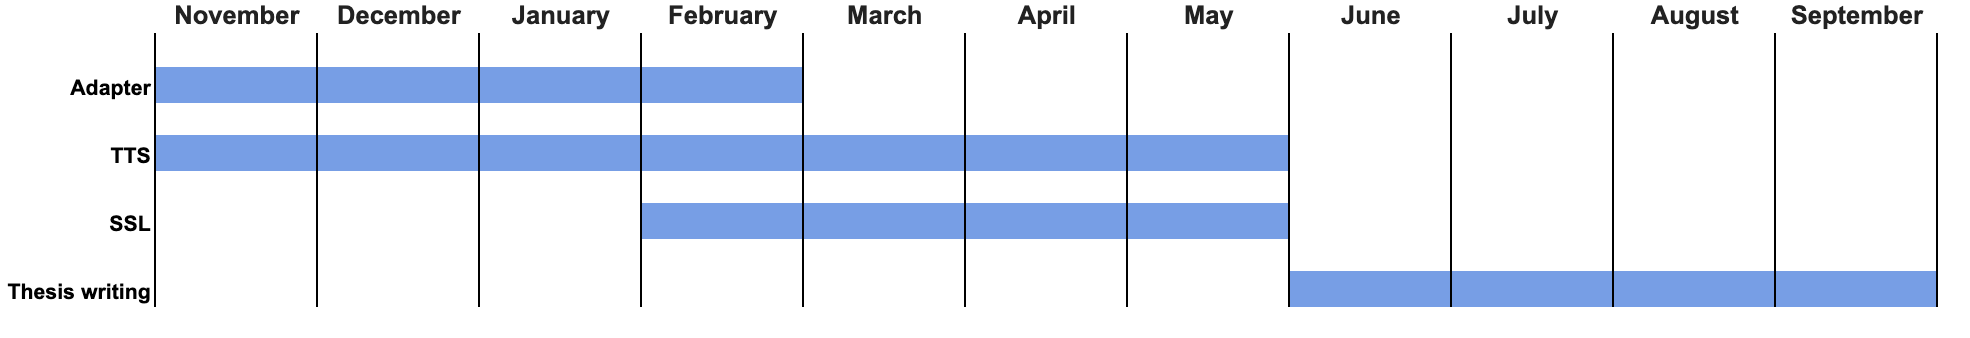
\includegraphics[width=1\textwidth]{imgs/Timeline.png}
    \caption{Proposed timeline - November 2022 - September 2023.}
    \label{fig:timeline}
\end{figure}